\documentclass[8pt]{beamer}

\usetheme{Copenhagen}
\usecolortheme{beaver}
\usepackage[small,center]{caption}
\usepackage{times}
\usefonttheme{structurebold}
\usepackage[english]{babel}
\usepackage{pgf,pgfarrows,pgfnodes,pgfautomata,pgfheaps}
\usepackage{amsmath,amssymb}
\usepackage{amsxtra}

\usepackage{caption}

\newcommand{\leftd}[1]{{\color{red} \bar{#1}}}
\newcommand{\interface}[2]{{\color{blue}{#1}_I(#2)}}
\newcommand{\leftdd}[2]{{\color{red} \bar{#1}(\bar{#2})}}
\newcommand{\leftFourier}[1]{{\color{red} \hat{#1}}}
\newcommand{\leftFourierTwo}[2]{{\color{red} \hat{#1}(\hat{#2})}}
\newcommand{\half}{\dfrac{1}{2}}
\newcommand{\divergence}{\mathrm{div}}

\newcommand*{\vcenterimage}[1]{\vcenter{\hbox{\includegraphics[width=2in]{#1}}}}
\newcommand*{\vcenterarrow}{\vcenter{\hbox{$\Longrightarrow$}}}


\definecolor{RPIred}{rgb}{ 0.87,0.12, 0.20}
\definecolor{ballblue}{rgb}{0.13, 0.67, 0.8}
\definecolor{lightgray}{rgb}{0.83, 0.83, 0.83}
\setbeamercolor{block title}{bg=lightgray,fg=RPIred}
\setbeamercolor{block body}{bg=white,fg=black}
\setbeamercovered{dynamic}
\setbeamercolor*{item}{fg=RPIred}

\captionsetup[subfigure]{labelformat=empty}
\captionsetup[figure]{labelformat=empty}
\setbeamertemplate{navigation symbols}{}
\setbeamertemplate{footline}[frame number]
\begin{document}

\frame{
\title{\Large Wave-Fluid Coupling with a Partitioned Algorithm}

\author{{\Large David Wells \\\vspace{0.1in} Rensselaer Polytechnic Institute}\\
\vspace{0.2in} {In collaboration with:\\{}J. W. Banks, F. Li}}

\date{August 11, 2016\\{} Nonlinear Waves and Coherent Structures}

\begin{figure}[h]
\centering
\includegraphics[width=1.5in]{RPI_letterhead.pdf}
 \end{figure}%

\vspace{-0.2in}
\titlepage
}

\begin{frame}
    \frametitle{Outline}
    \begin{itemize}
    \item[$\blacksquare$]  Definitions and Goals                              \\
    \item[$\blacksquare$]  Governing Equations                                \\
    \item[$\blacksquare$]  Added Mass Partition (AMP) Scheme                  \\
    \item[$\blacksquare$]  Finite Element Scheme                              \\
    \item[$\blacksquare$]  Numerical Results                                  \\
    \item[$\blacksquare$]  Summary                                            \\
    \end{itemize}
\end{frame}

\begin{frame}
    \frametitle{Physical Problem}
    Efficient, energy conserving finite element algorithms for wave problems are
    well-known. What happens when the wave is forced by a fluid?

    \begin{figure}
        \centering
        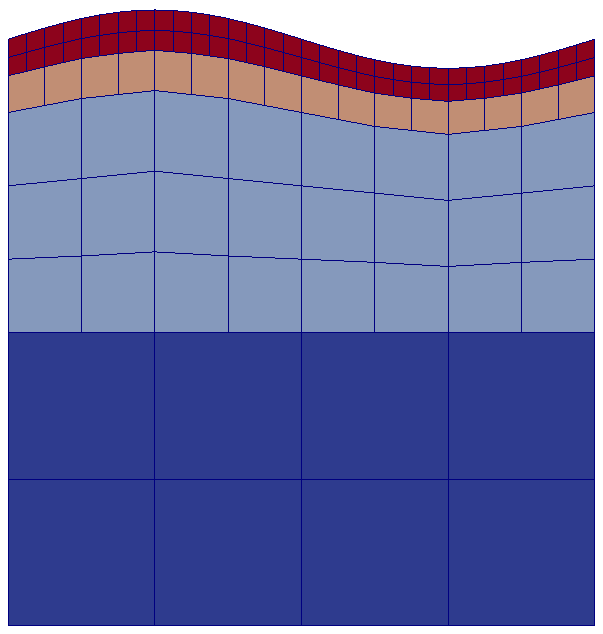
\includegraphics[width=2.25in]{refined-roof-wave.png}

        \caption{Depiction of physical setup: an elastic solid, governed by a
        wave (or beam equation), deforms in the presence of a fluid. The colors
        correspond to grid refinement levels.}
    \end{figure}
\end{frame}

\begin{frame}
    \frametitle{Partitioned Methods}
    \emph{Partitioned Methods} couple a fluid and structure solver along a
    specified interface. They are an alternative option to \emph{monolithic
    solvers}, which advance both the structure and the fluid in one joint
    system.
\end{frame}

\begin{frame}
    \frametitle{Goals \& Dreams}
    \begin{itemize}
        \item Reuse existing fluid and structure codes (without complete
              rewrites)
        \item Reasonable time step constraints
        \item No need for subiterations (\(O(10)\) to \(O(100)\)) for stability
        \item Arbitrarily high order accuracy
    \end{itemize}
\end{frame}

\begin{frame}
    \frametitle{Governing Equations}
    thin shell, i.e., a beam:
    \begin{equation}
        \leftd{u}_{tt} = \leftd{s} \leftd{u}_{xx} - \leftd{a} \leftd{u}_{xxxx}
        + \leftd{f}
    \end{equation}
    \pause
    \begin{align}
        \leftd{u}_t              &= \leftd{v}                                 \\
        \leftd{\rho} \leftd{v}_t &= \leftdd{L}{u} + \leftd{b} + \leftd{f}     \\
        \leftdd{L}{u}            &= \leftd{s} \leftd{u}_{xx}
        - \leftd{a} \leftd{u}_{xxxx}
    \end{align}
\end{frame}

\begin{frame}
    \frametitle{Governing Equations}
    incompressible fluid:
    \begin{align}
        \rho \vec{v}_t &= \divergence \sigma + \vec{f}                        \\
        \sigma &= -p I + 2 \nu \varepsilon(v)                                 \\
        \varepsilon(\vec{v})_{ij} &= \dfrac{1}{2}
        \left(
        \dfrac{\partial v_i}{\partial x_j} +
        \dfrac{\partial v_j}{\partial x_i}
        \right)                                                               \\
        \divergence \vec{v} &= 0
    \end{align}

    \pause
    coupling:
    \begin{align}
        v &= \leftd{v} \text{ (at the interface)}                             \\
        \leftd{b} &= -\sigma n.
    \end{align}
    \pause
    Physically motivated BCs: no jump in velocity, no jump in stress.
\end{frame}

\begin{frame}
    \frametitle{Governing Equations}
    The physical boundary conditions are a source of instability when the beam
    is very light.

    \begin{figure}
        \centering
        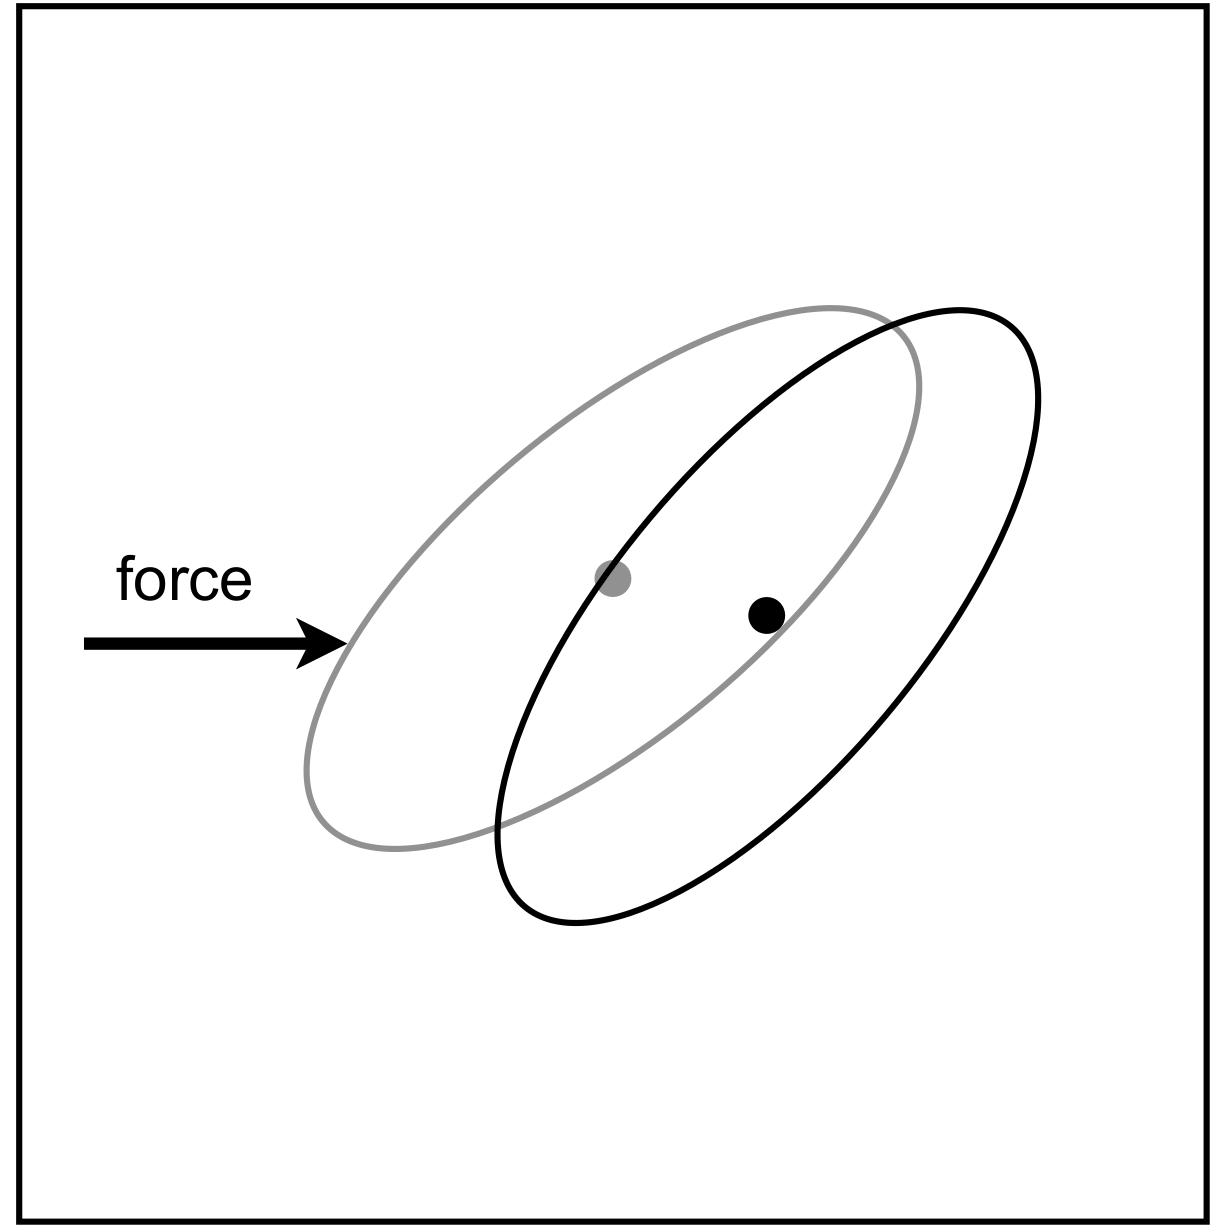
\includegraphics[width=2.25in]{left.png}

        \caption{A solid moving in a vacuum displaces no mass.}
    \end{figure}
\end{frame}

\begin{frame}
    \frametitle{Governing Equations}
    The physical boundary conditions are a source of instability when the beam
    is very light.

    \begin{figure}
        \centering
        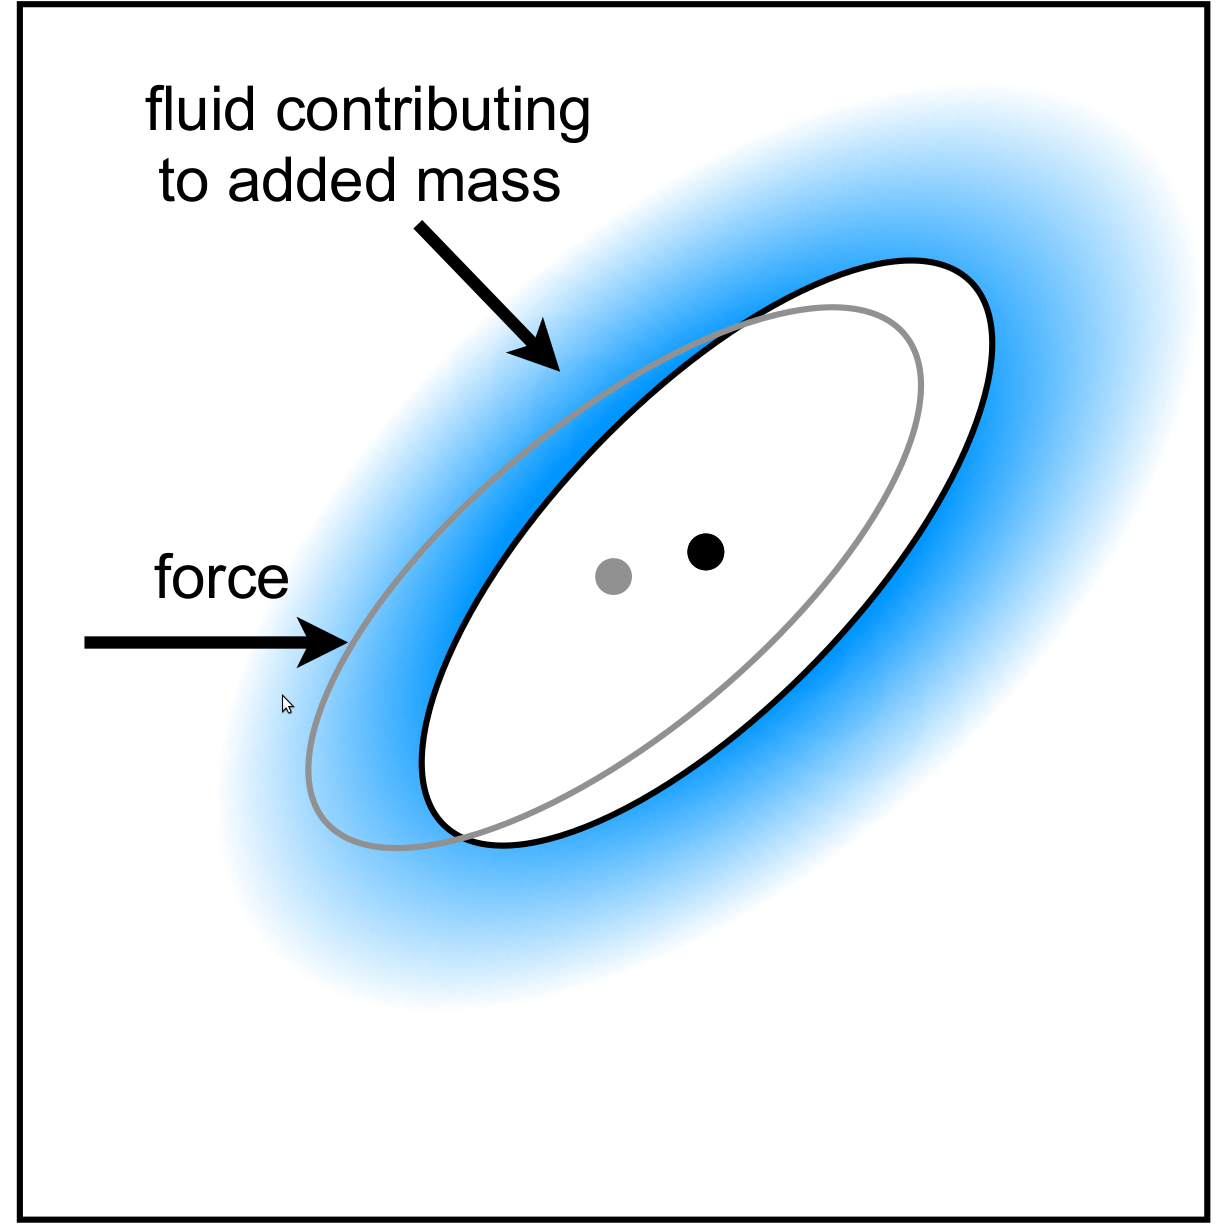
\includegraphics[width=2.25in]{right.png}

        \caption{A solid moving in a fluid must displace and entrain part of the
        fluid.}
    \end{figure}
\end{frame}

\begin{frame}
    \frametitle{Previous Work}
    Most of the work in our group has been done in a finite difference setting.
    \begin{figure}
        \centering

        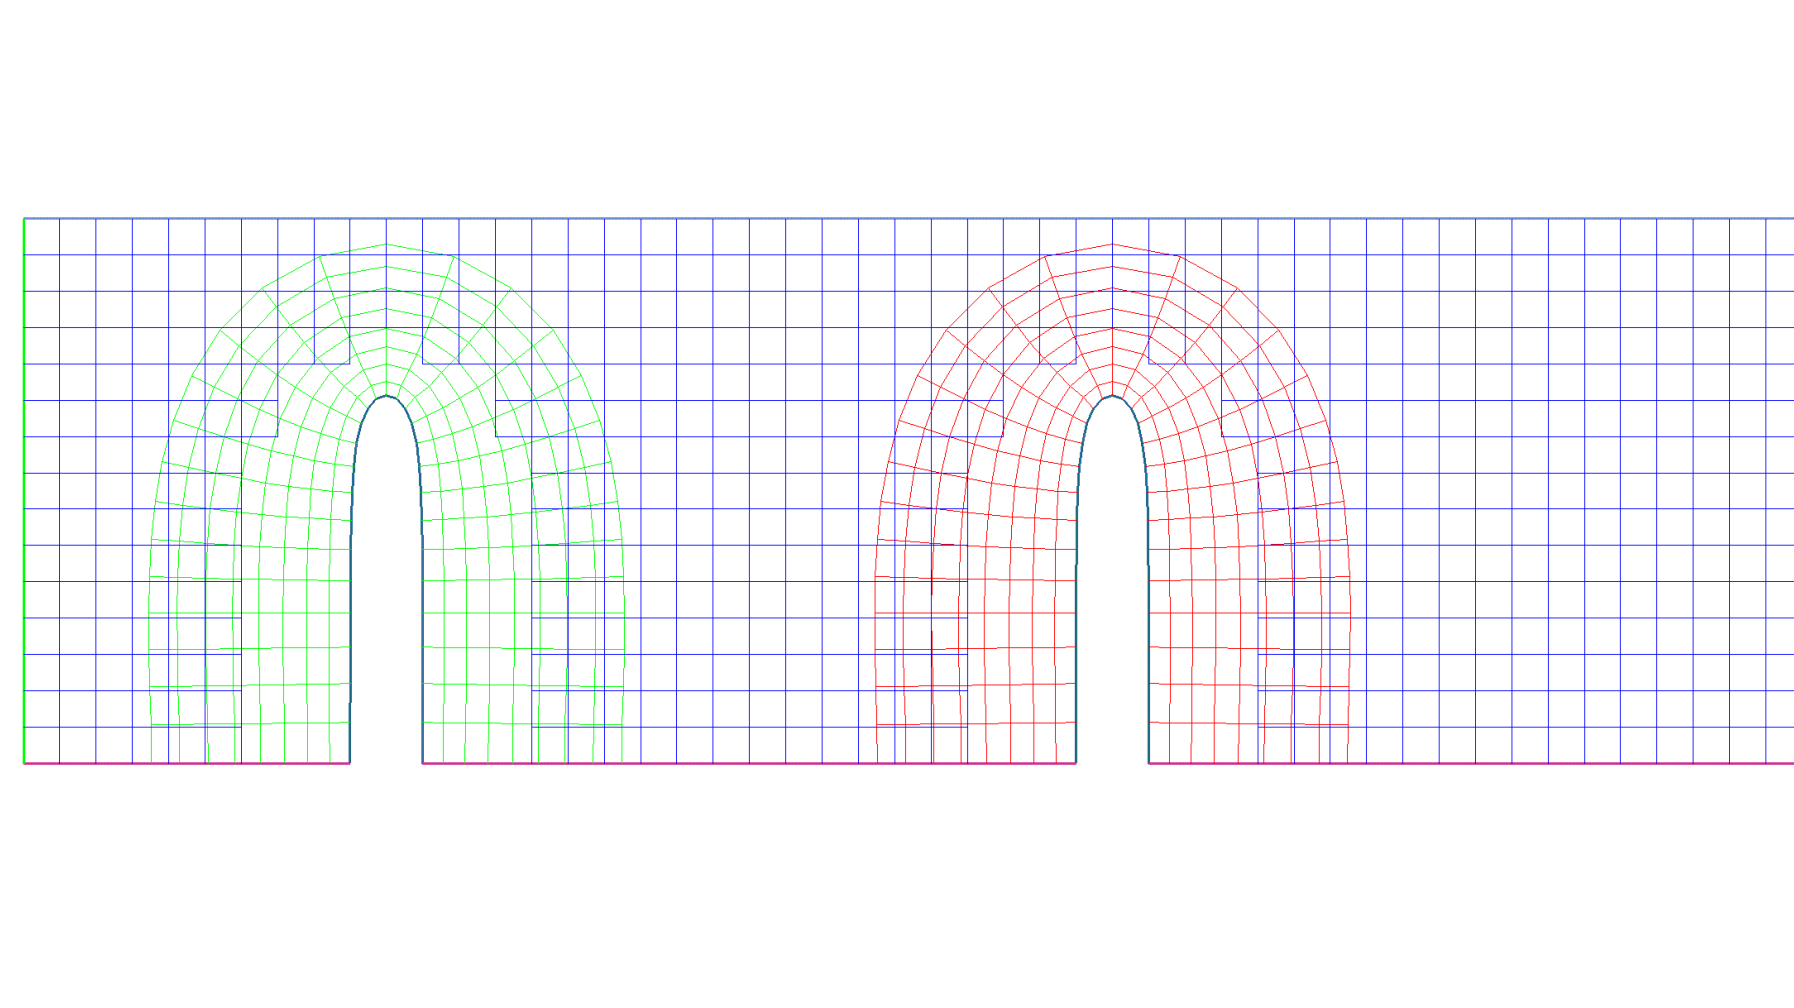
\includegraphics[width=3in]{longfei.png}

        \caption{Coarse grid of a channel with two protruding beams. Curvilinear
        grids describe the domain near the structures while the background
        Cartesian grid describes most of the domain.}
    \end{figure}
\end{frame}

\begin{frame}
    \frametitle{Traditional Coupling}
    \emph{Traditional Coupling} refers to taking the velocity from the beam and
    stress from the fluid.

    With some simplifying assumptions on the fluid (periodic in the non-shell
    direction, zero viscosity) we can explicitly compute the mode-dependent
    added mass \cite{amp-incompressible, causin-gerbeau-nobile-2010}:
    \begin{equation}
        M_{a,k} = \dfrac{\rho L}{2 \pi k} \coth(2 \pi k H / L)
    \end{equation}
    where \(H\) is the height of the fluid domain and \(L\) is the length (the
    beam is at the \(y = H\) boundary).

    \pause
    By a result from von Neumann polynomials the traditional scheme is only
    stable if
    \begin{align}
        M_a &< \leftd{\rho} \leftd{h}                                         \\
        \Delta t^2 &< 4 \dfrac{\leftd{\rho} \leftd{h}}{\leftd{\mathcal{L}}}
        \left[1 - \dfrac{M_a}{\leftd{\rho} \leftd{h}}\right]
    \end{align}
    where \(\leftd{\rho}\), \(\leftd{h}\), and \(\leftd{\mathcal{L}}\) are
    physical beam constants. The time stepping algorithms are backward Euler for
    the fluid and leapfrog for the beam.
\end{frame}

\begin{frame}
    \frametitle{AMP Coupling}
    Some beams are sufficiently light that (for the simplified model) that there
    is no stable time step choice with the traditional scheme.

    \begin{align}
        \leftd{\rho} \leftd{h} \leftd{v_t}
        &= \leftdd{\mathcal{L}}{u} + \leftd{f} - \sigma n
        \quad \text{ (beam equation)}                                         \\
        \leftd{\rho} \leftd{h} v_t
        &= \leftdd{\mathcal{L}}{u} + \leftd{f} - \sigma n
        \quad \text{ (equal acceleration)}                                    \\
        \dfrac{\leftd{\rho} \leftd{h}}{\rho} \divergence(\sigma)
        + \dfrac{\leftd{\rho} \leftd{h}}{\rho} f
        &= \leftdd{\mathcal{L}}{u} + \leftd{f} - \sigma n
        \quad \text{ (Stokes equations)}
    \end{align}
    or, more simply
    \begin{equation}
        \sigma n + \dfrac{\leftd{\rho} \leftd{h}}{\rho} \divergence(\sigma)
        = \leftdd{\mathcal{L}}{u}
        + \leftd{f}
        - \dfrac{\leftd{\rho} \leftd{h}}{\rho} f.
    \end{equation}
\end{frame}

\begin{frame}
    \frametitle{AMP Coupling}
    For the same model problem we now get a time step constraint (again by von
    Neumann polynomials) of
    \begin{equation}
        \Delta t < 2
        \sqrt{\dfrac{\leftd{\rho} \leftd{h} (1 + M_a)}{\leftd{\mathcal{L}}}}
    \end{equation}
\end{frame}

\begin{frame}
    \frametitle{What does this mean for finite elements?}
    An open area: compatibility boundary conditions (using the PDE at the
    boundary) is much more common for finite differences than finite elements.

    \pause
    \vspace{0.5in}
    After integrating by parts over the domain \(\Omega\):
    \begin{align}
        \rho (\varphi, \vec{v}_t) &= -(\nabla \varphi, \sigma)
        + (\varphi, \sigma n)_{\partial \Omega}
        + (\varphi, f)                                                        \\
        (q, \divergence(v)) &= 0
    \end{align}

    We replace the traction with second derivatives. This will make the
    energy estimate harder and probably won't work for classic FEM:
    \begin{equation}
        (\varphi, \sigma n)_{\partial \Omega} = \left(\varphi,
        - \dfrac{\leftd{\rho} \leftd{h}}{\rho} \divergence(\sigma)
        + \leftdd{\mathcal{L}}{u}
        + \leftd{f}
        - \dfrac{\leftd{\rho} \leftd{h}}{\rho} f\right)_{\partial \Omega}
    \end{equation}
\end{frame}

\begin{frame}
    \frametitle{What does this mean for finite elements?}
    Simplifications:
    \begin{itemize}
        \item Only enforce this AMP condition in the normal direction (e.g., use
              Dirichlet conditions tangentially)
        \item Assume that the beam solution is already known, i.e., enforce
              \begin{equation}
                  \sigma n n^T + \divergence(\sigma) n^T = g
              \end{equation}
              on the boundary.
    \end{itemize}
\end{frame}

\begin{frame}
    \frametitle{\(2D\) Numerical Experiments}
    \begin{itemize}
        \item \(Q^3-Q^2\) elements
        \item \(\Delta x = 1/50\)
        \item Unit square: the AMP condition is enforced along the top
        \item Velocity-divergence form
        \item Trapezoid rule time step
        \item \(\Delta t = \Delta x^2\)
    \end{itemize}
    with exact solution
    \begin{align}
        \psi(t, x, y) &= t y^2                                                \\
        p(t, x, y)    &= t x y
    \end{align}
\end{frame}

\begin{frame}
    \frametitle{\(2D\) Numerical Experiments}
    \begin{figure}
        \centering
        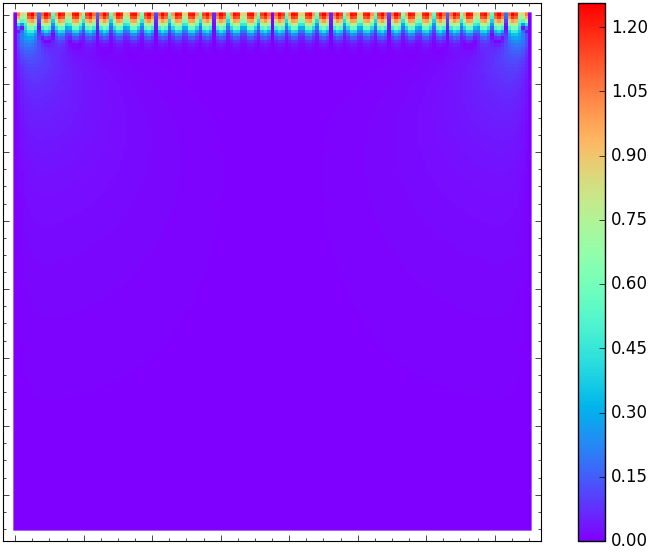
\includegraphics[width=3in]{v1-10.png}

        \caption{Magnitude in the error after ten time steps. As anticipated the
        scheme doesn't work.}
    \end{figure}
\end{frame}

\begin{frame}
    \frametitle{\(2D\) Numerical Experiments}
    \begin{figure}
        \centering
        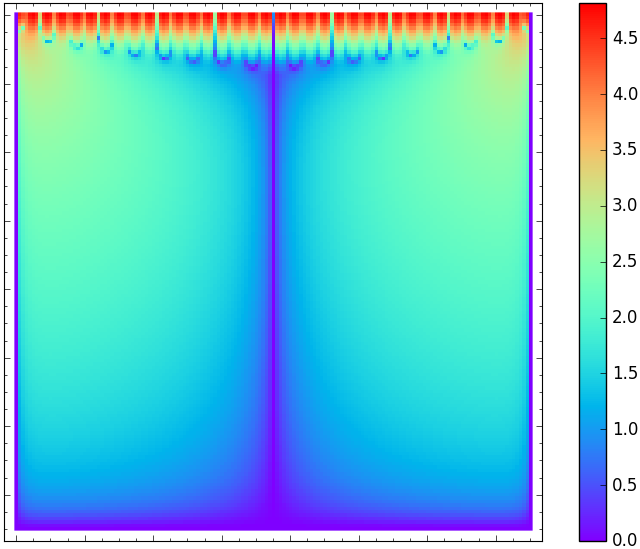
\includegraphics[width=3in]{v1-12.png}

        \caption{Magnitude in the error after twelve time steps.}
    \end{figure}
\end{frame}

\begin{frame}
    \frametitle{Dealing with the instability}
    Implementing the AMP boundary, even with integration by parts, requires
    derivative information at the boundary which may not exist: a workaround is
    to use elements with some derivative information.

    \begin{figure}
        \begin{equation*}
            \vcenterimage{lagrange-quadratics.png}
            \vcenterarrow
            \vcenterimage{hermite-quadratics.png}
        \end{equation*}
    \end{figure}
\end{frame}

\begin{frame}
    \frametitle{Dealing with the instability}
    \begin{align}
        \begin{pmatrix}
            \hat{u} \\ \hat{v}
        \end{pmatrix}_t
        =
        \begin{pmatrix}
            i k & \dfrac{\partial}{\partial y}
        \end{pmatrix}
        \cdot
        \left[
        \begin{pmatrix}
            -\hat{p} \vphantom{\dfrac{1}{2}} & 0                              \\
            0 \vphantom{\dfrac{1}{2}}        & -\hat{p}
        \end{pmatrix}
        +
        2 \nu
        \begin{pmatrix}
            i k \hat{u} & \dfrac{1}{2} \left(\hat{u}_y + i k \hat{v}\right)   \\
            \dfrac{1}{2} \left(\hat{u}_y + i k \hat{v}\right) & \hat{v}_y
        \end{pmatrix}
        \right]
        +
        \begin{pmatrix}
            \hat{f}_0 \vphantom{\dfrac{1}{2}}                                 \\
            \hat{f}_1 \vphantom{\dfrac{1}{2}}
        \end{pmatrix}
    \end{align}
    where in this context \(i k\) is the differential operator in \(x\). This
    leads to the weak form
    \begin{align}
        (\varphi_0, \hat{u})_t
        &=
        -2 \nu k^2 (\varphi_0, \hat{u})
        - \nu (\varphi_{0,y}, \hat{u}_y + i k \hat{v})
        - i k (\varphi_0, p)
        + (\varphi_0, \hat{f}_0)                                              \\
        (\varphi_1, \hat{v})_t
        &=
        -2 \nu (\varphi_{1,y}, \hat{v}_y)
        + \nu (\varphi_1, i k \hat{u}_y - k^2 \hat{v})
        + (\varphi_{1,y}, p)                                                  \\
        &\phantom{=} + (\varphi_1, \hat{f}_1)
        + \varphi_1(1) (2 \nu \hat{v}_y(1) - \hat{p}(1))
        \nonumber                                                             \\
        (q, i k \hat{u} + \hat{v}_y)
        &= 0.
    \end{align}

    \pause
    AMP boundary condition in 1D:
    \begin{equation}
        2 \nu \varphi_1(1) \hat{v}_y(1) - \varphi_1(1) \hat{p}(1)
        = \hat{g}(1) - \nu (-k^2 \hat{v}(1) - i k \hat{u}_y(1)) + \hat{p}_y(1)
    \end{equation}
\end{frame}

\begin{frame}
    \frametitle{\(1D\) Numerical Experiments}
    Discretization:
    \begin{itemize}
        \item \(Q^3\)-\(Q^2\) pair for velocity-pressure
        \item Trapezoid rule in time, \(\Delta t = \Delta x^2\)
        \item Beam is a point (e.g., an ODE)
    \end{itemize}
    \pause
    Method of manufactured solutions:
    \begin{align}
        \psi(t, y) &= t \sin(3.3 y t) \cos(3 y) \exp(4 y)                     \\
           p(t, y) &= t y (5 - y)^2 \exp(-3 y) \sin(5 t)
    \end{align}
\end{frame}

\begin{frame}
    \frametitle{Dealing with the instability}
    \begin{figure}
        \centering
        \begin{tabular}{| l | l | l | l | l | l |}
            \hline
            \(k\) & \texttt{n\_cells} &
            \(\hat{p}\) error & \(\hat{u}\) error &
            \(\hat{p}\) rate & \(\hat{u}\) rate                               \\
            \hline
            0 & 10 & 3.16e-03 & 4.97e-03 & -    & -                           \\
            0 & 20 & 1.07e-03 & 3.13e-04 & 1.55 & 3.98                        \\
            0 & 30 & 5.12e-04 & 6.20e-05 & 1.83 & 3.99                        \\
            0 & 40 & 2.97e-04 & 1.96e-05 & 1.89 & 3.99                        \\
            0 & 50 & 1.93e-04 & 8.05e-06 & 1.92 & 3.99                        \\
            0 & 60 & 1.35e-04 & 3.88e-06 & 1.94 & 3.99                        \\
            0 & 70 & 1.00e-04 & 2.09e-06 & 1.95 & 3.99                        \\
            0 & 80 & 7.72e-05 & 1.22e-06 & 1.96 & 3.99                        \\
            0 & 90 & 6.12e-05 & 7.67e-07 & 1.96 & 3.99                        \\
            \hline
            1 & 10 & 4.21e-00 & 2.40e-01 & -    & -                           \\
            1 & 20 & 5.91e-01 & 3.51e-02 & 2.83 & 2.77                        \\
            1 & 30 & 1.81e-01 & 1.09e-02 & 2.91 & 2.88                        \\
            1 & 40 & 7.76e-02 & 4.71e-03 & 2.94 & 2.91                        \\
            1 & 50 & 4.01e-02 & 2.44e-03 & 2.95 & 2.93                        \\
            1 & 60 & 2.33e-02 & 1.42e-03 & 2.96 & 2.95                        \\
            1 & 70 & 1.47e-02 & 9.05e-04 & 2.97 & 2.95                        \\
            1 & 80 & 9.92e-03 & 6.09e-04 & 2.97 & 2.96                        \\
            1 & 90 & 6.98e-03 & 4.29e-04 & 2.97 & 2.96                        \\
            \hline
        \end{tabular}

        \caption{Rates of convergence for the first and second wavenumbers. The
        method is stable, but loses an order of convergence.}
    \end{figure}
\end{frame}

\begin{frame}
    \frametitle{Equation for a ``\(0\) dimensional'' beam}
    If we Fourier transform the beam equation we get an ODE:
    \begin{align}
        \leftFourier{u}_t              &= \leftFourier{v}                     \\
        \leftd{\rho} \leftFourier{v}_t &= \leftFourierTwo{L}{u}
        - \sigma n + \leftFourier{f} \leftFourier{L}                          \\
        \leftFourier{L} &= -\leftd{s} k^2 - \leftd{a} k^4
    \end{align}
\end{frame}

\begin{frame}
    \frametitle{Convergence for a somewhat light beam}
    For \(\leftd{\rho} = 100\):
    \begin{figure}
        \centering
        \begin{tabular}{| l | l | l | l | l | l | l | l |}
            \hline
            \(k\) & \texttt{n\_cells} &
            \(\hat{p}\) error & \(\hat{v}\) error & \(\leftFourier{v}\) error &
            \(\hat{p}\) rate & \(\hat{v}\) rate & \(\leftFourier{v}\) rate    \\
            \hline
            0 & 10 & 2.89e-01 & 4.97e-03 & 2.87e-04 & -    & -    & -         \\
            0 & 20 & 1.06e-01 & 3.13e-04 & 1.05e-04 & 1.44 & 3.98 & 1.44      \\
            0 & 30 & 5.10e-02 & 6.20e-05 & 5.05e-05 & 1.81 & 3.99 & 1.81      \\
            0 & 40 & 2.96e-02 & 1.96e-05 & 2.93e-05 & 1.89 & 3.99 & 1.89      \\
            0 & 50 & 1.92e-02 & 8.05e-06 & 1.91e-05 & 1.92 & 3.99 & 1.92      \\
            0 & 60 & 1.35e-02 & 3.88e-06 & 1.34e-05 & 1.93 & 3.99 & 1.93      \\
            0 & 70 & 1.00e-02 & 2.09e-06 & 9.93e-06 & 1.95 & 3.99 & 1.95      \\
            0 & 80 & 7.71e-03 & 1.22e-06 & 7.65e-06 & 1.95 & 3.99 & 1.95      \\
            0 & 90 & 6.12e-03 & 7.67e-07 & 6.07e-06 & 1.96 & 3.99 & 1.96      \\
            \hline
            1 & 10 & 1.68e+01 & 7.97e-01 & 1.21e-02 & -    & -    & -         \\
            1 & 20 & 2.52e+00 & 1.26e-01 & 2.01e-03 & 2.73 & 2.65 & 2.59      \\
            1 & 30 & 7.89e-01 & 4.05e-02 & 6.59e-04 & 2.86 & 2.81 & 2.75      \\
            1 & 40 & 3.42e-01 & 1.77e-02 & 2.92e-04 & 2.90 & 2.87 & 2.82      \\
            1 & 50 & 1.78e-01 & 9.27e-03 & 1.54e-04 & 2.92 & 2.90 & 2.86      \\
            1 & 60 & 1.04e-01 & 5.44e-03 & 9.09e-05 & 2.94 & 2.92 & 2.89      \\
            1 & 70 & 6.60e-02 & 3.46e-03 & 5.81e-05 & 2.95 & 2.93 & 2.90      \\
            1 & 80 & 4.44e-02 & 2.33e-03 & 3.93e-05 & 2.95 & 2.94 & 2.92      \\
            1 & 90 & 3.13e-02 & 1.65e-03 & 2.78e-05 & 2.96 & 2.95 & 2.93      \\
            \hline
        \end{tabular}
        \caption{Rates of convergence for the first wave number and second wave
        numbers. The lower pressure convergence rate damages the beam's
        convergence rate when \(k = 0\).}
    \end{figure}
\end{frame}

\begin{frame}
    \frametitle{Convergence for a \emph{very} light beam}
    For \(\leftd{\rho} = 2\):
    \begin{figure}
        \centering
        \begin{tabular}{| l | l | l | l | l | l | l | l |}
            \hline
            \(k\) & \texttt{n\_cells} &
            \(\hat{p}\) error & \(\hat{v}\) error & \(\leftFourier{v}\) error &
            \(\hat{p}\) rate & \(\hat{v}\) rate & \(\leftFourier{v}\) rate    \\
            \hline
            0 & 10 & 5.93e-03 & 4.97e-03 & 1.04e-04 & -    & -    & -         \\
            0 & 20 & 2.13e-03 & 3.13e-04 & 1.04e-04 & 1.47 & 3.98 & 1.40      \\
            0 & 30 & 1.02e-03 & 6.20e-05 & 5.04e-05 & 1.82 & 3.99 & 1.80      \\
            0 & 40 & 5.92e-04 & 1.96e-05 & 2.93e-05 & 1.89 & 3.99 & 1.88      \\
            0 & 50 & 3.85e-04 & 8.05e-06 & 1.90e-05 & 1.92 & 3.99 & 1.91      \\
            0 & 60 & 2.70e-04 & 3.88e-06 & 1.34e-05 & 1.94 & 3.99 & 1.93      \\
            0 & 70 & 2.00e-04 & 2.09e-06 & 9.93e-06 & 1.95 & 3.99 & 1.94      \\
            0 & 80 & 1.54e-04 & 1.22e-06 & 7.64e-06 & 1.95 & 3.99 & 1.95      \\
            0 & 90 & 1.22e-04 & 7.67e-07 & 6.06e-06 & 1.96 & 3.99 & 1.96      \\
            \hline
            1 & 10 & 7.00e-00 & 3.86e-01 & 7.25e-02 & -    & -    & -         \\
            1 & 20 & 9.93e-01 & 5.72e-02 & 7.25e-02 & 2.81 & 2.75 & 2.72      \\
            1 & 30 & 3.05e-01 & 1.78e-02 & 2.28e-02 & 2.90 & 2.87 & 2.84      \\
            1 & 40 & 1.31e-01 & 7.73e-03 & 9.95e-03 & 2.93 & 2.91 & 2.89      \\
            1 & 50 & 6.79e-02 & 4.01e-03 & 5.18e-03 & 2.95 & 2.93 & 2.91      \\
            1 & 60 & 3.95e-02 & 2.34e-03 & 3.04e-03 & 2.96 & 2.94 & 2.93      \\
            1 & 70 & 2.50e-02 & 1.48e-03 & 1.93e-03 & 2.96 & 2.95 & 2.94      \\
            1 & 80 & 1.68e-02 & 1.00e-03 & 1.30e-03 & 2.97 & 2.96 & 2.95      \\
            1 & 90 & 1.18e-02 & 7.07e-04 & 9.19e-04 & 2.97 & 2.96 & 2.95      \\
            \hline
        \end{tabular}
        \caption{Rates of convergence for the first and second wave numbers. The
        rates change from \(k = 0\) to \(k = 1\) again.}
    \end{figure}
\end{frame}

\begin{frame}
    \frametitle{Summary}
    \begin{itemize}
        \item The AMP boundary condition is known to work better for light beams.
        \item Traditional FEM breaks down with the AMP BC.
        \item Hermite element approach appears promising.
    \end{itemize}
\end{frame}

\begin{frame}
    \begin{center}
    \textcolor{RPIred}{\Huge Thank You!}
    \end{center}
\end{frame}

\begin{frame}[allowframebreaks]
    %This is the standard bibtex file
    %uncomment the following to include your bibliography
    \bibliographystyle{plain}
    \tiny
    {
    \bibliography{citations}
    }
\end{frame}
\end{document}
